\section{zesto-alloc.cpp File Reference}
\label{zesto-alloc_8cpp}\index{zesto-alloc.cpp@{zesto-alloc.cpp}}
{\tt \#include $<$limits.h$>$}\par
{\tt \#include \char`\"{}thread.h\char`\"{}}\par
{\tt \#include \char`\"{}zesto-core.h\char`\"{}}\par
{\tt \#include \char`\"{}zesto-opts.h\char`\"{}}\par
{\tt \#include \char`\"{}zesto-oracle.h\char`\"{}}\par
{\tt \#include \char`\"{}zesto-decode.h\char`\"{}}\par
{\tt \#include \char`\"{}zesto-alloc.h\char`\"{}}\par
{\tt \#include \char`\"{}zesto-exec.h\char`\"{}}\par
{\tt \#include \char`\"{}zesto-commit.h\char`\"{}}\par
{\tt \#include \char`\"{}ZPIPE-alloc.list\char`\"{}}\par


Include dependency graph for zesto-alloc.cpp:\nopagebreak
\begin{figure}[H]
\begin{center}
\leavevmode
\includegraphics[width=420pt]{zesto-alloc_8cpp__incl}
\end{center}
\end{figure}
\subsection*{Functions}
\begin{CompactItemize}
\item 
void {\bf alloc\_\-reg\_\-options} (struct {\bf opt\_\-odb\_\-t} $\ast$odb, struct {\bf core\_\-knobs\_\-t} $\ast${\bf knobs})
\item 
class {\bf core\_\-alloc\_\-t} $\ast$ {\bf alloc\_\-create} (const char $\ast$alloc\_\-opt\_\-string, struct {\bf core\_\-t} $\ast$core)
\end{CompactItemize}


\subsection{Function Documentation}
\index{zesto-alloc.cpp@{zesto-alloc.cpp}!alloc\_\-create@{alloc\_\-create}}
\index{alloc\_\-create@{alloc\_\-create}!zesto-alloc.cpp@{zesto-alloc.cpp}}
\subsubsection[{alloc\_\-create}]{\setlength{\rightskip}{0pt plus 5cm}class {\bf core\_\-alloc\_\-t}$\ast$ alloc\_\-create (const char $\ast$ {\em alloc\_\-opt\_\-string}, \/  struct {\bf core\_\-t} $\ast$ {\em core})}\label{zesto-alloc_8cpp_d5e0575b7db14c11053d5da87dab1708}




Definition at line 116 of file zesto-alloc.cpp.

References fatal().

Referenced by sim\_\-post\_\-init().

Here is the caller graph for this function:\nopagebreak
\begin{figure}[H]
\begin{center}
\leavevmode
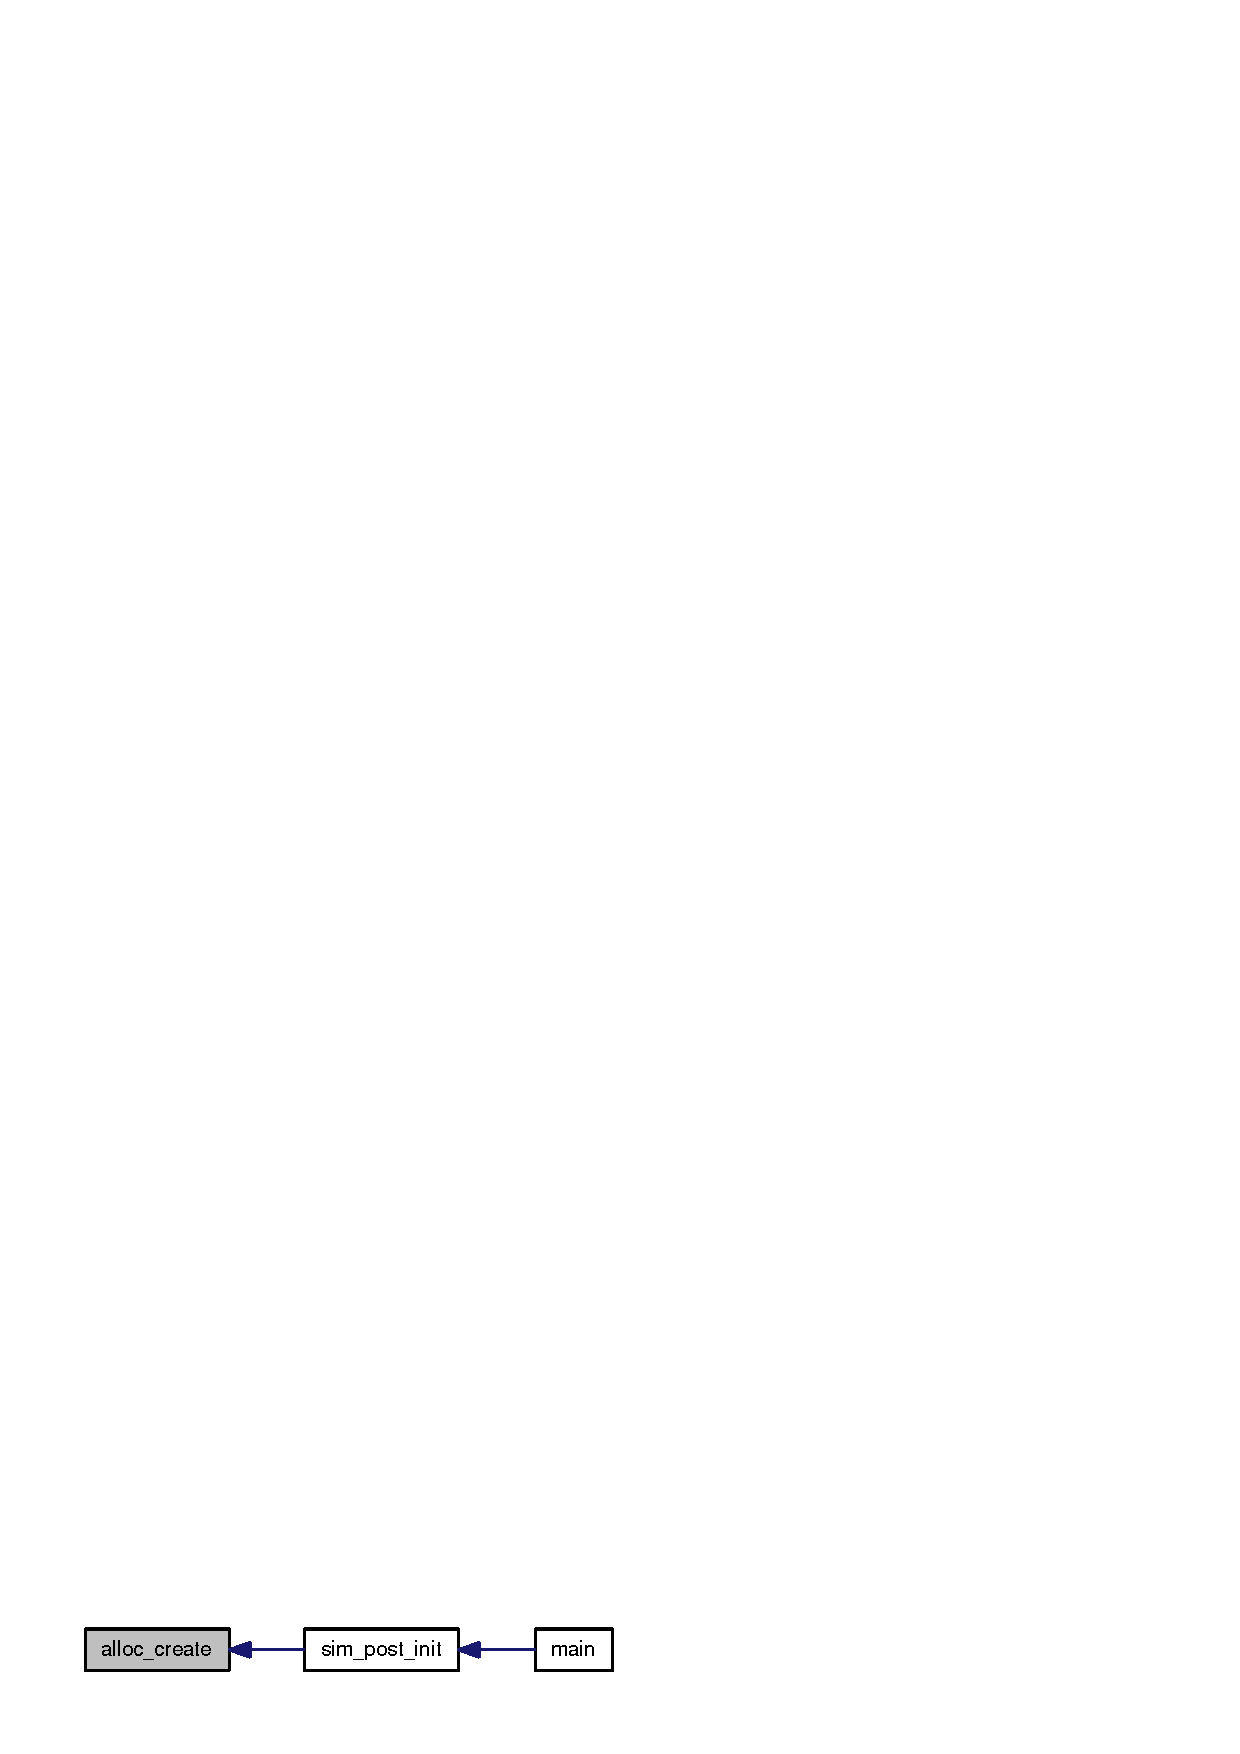
\includegraphics[width=149pt]{zesto-alloc_8cpp_d5e0575b7db14c11053d5da87dab1708_icgraph}
\end{center}
\end{figure}
\index{zesto-alloc.cpp@{zesto-alloc.cpp}!alloc\_\-reg\_\-options@{alloc\_\-reg\_\-options}}
\index{alloc\_\-reg\_\-options@{alloc\_\-reg\_\-options}!zesto-alloc.cpp@{zesto-alloc.cpp}}
\subsubsection[{alloc\_\-reg\_\-options}]{\setlength{\rightskip}{0pt plus 5cm}void alloc\_\-reg\_\-options (struct {\bf opt\_\-odb\_\-t} $\ast$ {\em odb}, \/  struct {\bf core\_\-knobs\_\-t} $\ast$ {\em knobs})}\label{zesto-alloc_8cpp_958130a4752ea3e0b57acdab47cff685}




Definition at line 87 of file zesto-alloc.cpp.

References core\_\-knobs\_\-t::alloc, core\_\-knobs\_\-t::depth, core\_\-knobs\_\-t::drain\_\-flush, opt\_\-reg\_\-flag(), opt\_\-reg\_\-int(), and core\_\-knobs\_\-t::width.